%% ----------------------------------------------------------------------------
% CVG SA/MA thesis template
%
% Created 03/08/2024 by Tobias Fischer
%% ----------------------------------------------------------------------------
\newpage
\chapter{Experiments}

In this section, we detail experimental methods and results for the generation of the ScanSG dataset and the proposed ScanSG-Transformer model.

\section{Scene Graph Generation}

In order to train a successful 3D-VQA model, we must ensure that its input data, namely generated scene graphs and questions, are of high quality. This section empirically evaluates the impact of different design choices on the quality of the generated scene graphs. We evaluate the design choices for scene graph nodes and edges separately, and choose the best performing parameters for the proposed scene graph dataset. For scene graph nodes, we evaluate the effects of different cropping methods, k-values, and visibility scores on the quality of the node embeddings. For scene graph edges, we evaluate the impact of different threshold values on the quality of the edges in the scene graphs.

All experiments in this section are performed on a smaller subset of the dataset, consisting of 71 scenes, with a total of 2467 objects across scenes. This subset is also used for testing in section XXX.

\subsection{Node Construction}
We evaluate the impact of different cropping methods, k-values and visibility scores on the quality of the generated node CLIP-embeddings. The following paragraphs detail the methods and parameters considered for each of these design choices.

\bigskip \noindent
\textbf{Cropping method:}
We compare the impact of the following cropping methods on node embedding quality (illustrated in Figure XXX):
\begin{enumerate}
    \item A tight, rectangular crop around the object with all background pixels masked out. With this method, the object is centered in the image, and the background is removed. However, CLIP was trained on square images with no background removal. To adapt rectangular crops to CLIP, we use the resizing method described in the original CLIP paper [XXX]: the crop is resized to $224$ in its minimum dimension, and then randomly cropped to a $224 \times 224$ square.
    
    \item A tight, rectangular crop around the object with no further changes. With this method, the object is centered in the image. However, the background is not removed, meaning other surrounding objects could contribute to the embedding, and the image is not square. The rectangular crops are resized as in the original CLIP paper [XXX].
    
    \item A square crop centred around the object, resized to $224 \times 224$. With this method, the crop is square and correctly sized, and no further processing is needed. However, the background is not removed and the non-tight crop means other surrounding objects might contribute to the node embedding.
    
    \item A tight, rectangular crop, resized to $224 \times 224$. With this method, the crop is tight around the object (fewer surrounding objects included in the crop). However, the resized crops distort the image, and CLIP was not trained on distorted images.
\end{enumerate}

\begin{figure}[h!]
    \centering
    \begin{minipage}[b]{0.1\textwidth}
        \centering
        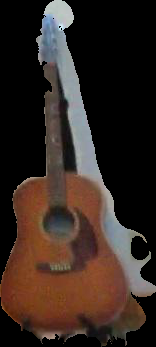
\includegraphics[width=\textwidth]{images/cropping_method_0.png}
        \caption{Caption 1}
    \end{minipage}
    \hspace{1em} % Adjust this to control the horizontal space between images
    \begin{minipage}[b]{0.1\textwidth}
        \centering
        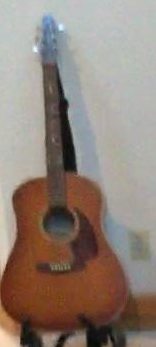
\includegraphics[width=\textwidth]{images/cropping_method_1.png}
        \caption{Caption 2}
    \end{minipage}
    \vspace{0em} % Adjust this to control the vertical space between rows
    \begin{minipage}[b]{0.1\textwidth}
        \centering
        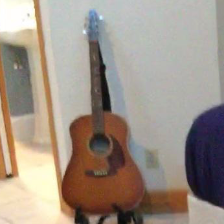
\includegraphics[width=\textwidth]{images/cropping_method_2.png}
        \caption{Caption 3}
    \end{minipage}
    \hspace{1em} % Adjust this to control the horizontal space between images
    \begin{minipage}[b]{0.1\textwidth}
        \centering
        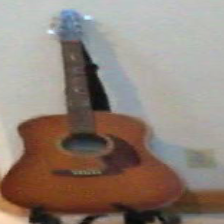
\includegraphics[width=\textwidth]{images/cropping_method_3.png}
        \caption{Caption 4}
    \end{minipage}
    \caption{Overall figure caption}
\end{figure}

\bigskip \noindent
\textbf{k-value:}
We also evaluate the impact of different k-values on the quality of the scene graph nodes. The k-value determines how many images of the object will be considered when generating the scene graph node. A higher value of k could result in a more accurate representation of the object, but could also introduce noise or inconsistencies as different views may have different different embeddings. We not that increasing the k-value highly increases the computational cost. It is therefore important to find the optimal k-value that balances these trade-offs. In this analysis we consider the following k-values: $k=1$, $k=3$, and $k=10$.

\bigskip \noindent
\textbf{Visibility score:}
\begin{enumerate}
    \item $s_1 = \frac{n}{w \times h} \times \frac{b}{8}$
    \item $s_2 = w_p \frac{n}{w \times h} + w_c \frac{b}{8}$ with $w_p = 1$, $w_c = 1$
    \item $s_2$ with $w_p = 1$, $w_c = 0$
    \item $s_2$ with $w_p = 0$, $w_c = 1$
\end{enumerate}

To evaluate the comparative quality of these cropping methods and k-values, we perform the following experiment: first, we generate scene graphs using each of the three cropping methods, with $k=1$, $k=3$ and $k=10$ respectively. We therefore have a total of 9 different scene graph node generation methods. Then, we CLIP-embed all the object labels in the scene, and calculate the similarity between the embeddings of the object crops and the embeddings of the object labels. For each object, we select the label with the highest similarity, and compare it to the ground truth label. We calculate the accuracy of the scene graph nodes for each of the 9 methods, and choose the best performing method for the final model.  Note that we only use semantic accuracy (since there is no context-awareness mechanism or learning in this experiment) to evaluate the quality of the scene graph nodes. The semantic accuracy is the percentage of nodes that are embedded closest to their label in the CLIP embedding space. We repeat this experiment for each visibility score listed above, keeping the cropping method and k-value constant. Tables XX shows the results of this experiment.

\begin{table}[h!]
    \centering
    \caption{}
    \begin{tabular}{l|lll|}
    \cline{2-4}
                                                   & \multicolumn{3}{c|}{\textbf{k-value}} \\ \hline
    \multicolumn{1}{|c|}{\textbf{Cropping method}} & 1        & 3       & 10               \\ \hline
    \multicolumn{1}{|l|}{Tight masked crop}        & 49.5     & 50.1    & 52.1             \\
    \multicolumn{1}{|l|}{Tight crop}               & 57.6     & 58.9    & 60.3             \\
    \multicolumn{1}{|l|}{Square crop}              & 57.1     & 58.3    & \textbf{62.2}    \\
    \multicolumn{1}{|l|}{Tight resized crop}       & 56.2     & 57.4    & 60.2             \\ \hline
    \end{tabular}
\end{table}
\begin{table}[h!]
    \centering
    \caption{}
    \begin{tabular}{|c|c|}
    \hline
    \textbf{Visibility Score} & \textbf{Accuracy} \\ \hline
    s1                       & 62.2               \\ \hline
    s2                        &                   \\ \hline
    s3                        &                   \\ \hline
    s4                        &                   \\ \hline
    \end{tabular}
\end{table}

\bigskip
\noindent
\textbf{Results and Interpretation}

Table XX shows some examples of inaccurate node embeddings. The table shows the crop of the object, the ground truth label, and the label with the highest similarity to the object crop. These inaccuracies are most often caused by other objects appearing in the object of interest's crop for the following reasons:
\begin{itemize}
    \item they occlude the object of interest (see floor example)
    \item they are contained within the object of interest (see doorframe example)
    \item they are similar to the object of interest (see shelf example)
    \item the object of interest is rectangular so a square crop includes other objects (see guitar case example)
\end{itemize}

\begin{table}[h]
    \centering
    \caption{}
    \begin{tabular}{|c|l|l|}
        \hline
        \textbf{Crop} & \textbf{Ground Truth Label} & \textbf{Most Similar Label} \\ \hline
        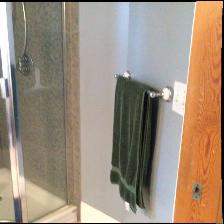
\includegraphics[width=1in]{images/wall.png} & Wall & Shower \\ \hline
        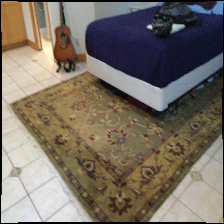
\includegraphics[width=1in]{images/floor.png} & Floor & Bed \\ \hline
        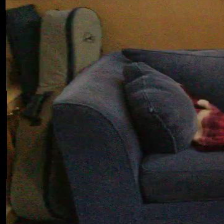
\includegraphics[width=1in]{images/guitar case.png} & Guitar Case & Couch \\ \hline
        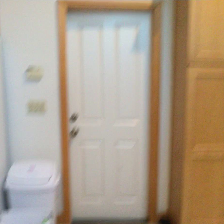
\includegraphics[width=1in]{images/doorframe.png} & Doorframe & Door \\ \hline
        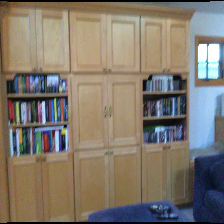
\includegraphics[width=1in]{images/shelf.png} & Shelf & Cabinet \\ \hline
    \end{tabular}
\end{table}

These examples highlight some inherent limitations of the CLIP method. However, we believe CLIP embeddings are still a good starting points as they offer a common embedding for the images in text, which is accurate in most cases.

The experiments also highlight the necessity of including some learning into the model, because the CLIP-embedding of the object is not very close to the CLIP-embedding of the object label. And this label task is easier than the question task, as shown in Figure XXX.


\subsection{Edge Construction}
Same model, same node embeddings (only change is the edges).

\begin{table}[h!]
    \centering
    \caption{accuracy (percent)}
    \begin{tabular}{|c|c|}
    \hline
    \multicolumn{1}{|l|}{\textbf{Threshold value (m)}} & \textbf{EM@1 (\%)} \\ \hline
    0.2                                                & \textbf{20.1}      \\ \hline
    0.5                                                & 14.6               \\ \hline
    0.8                                                & 9.8                \\ \hline
    Random edges                                       & 4.0                \\ \hline
    \end{tabular}
    \end{table}

Dense graphs perform better than sparse graphs. Cannot use no edges because then the scene structure is lost.
So these edges help the model learn.

We train GNN model on the scene graphs with different threshold values for the edges. We evaluate the performance of the model on the test set, and choose the best threshold value for the final sg dataset. We also compare the performance of the model with the best threshold value to the performance of the model with random edges. Table XXX shows the results of this experiment.

Simple GNN model -> show that chosen threshold is better than random edges.
Also show that edges can have a huge impact on the final answer --> must be chosen carefully.



\subsection{Edge Label Classification}


%%%%%%%%%%%%%%%%%%%%%%%%%%%%%%%%%%%% VQA %%%%%%%%%%%%%%%%%%%%%%%%%%%%%%%%%%
\newpage
\section{Visual Question Answering Model}

In this section, we assess the performance of each model described in section XXX on the ScanSG dataset. We evaluate the performance of the baseline model, the baseline + GNN model, the proposed ScanSG-GNN model, and the proposed ScanSG-Transformer model. The dataset split, evaluation metrics, and hyperparameters common to all models are described below. The specific details of each model are described in the relevant sections, such that the results can be reproduced.

\subsection{GraphVQA}


\subsection{Experimental Setup for Proposed Models}
\bigskip
\noindent \textbf{Dataset}
The train/test split from the original ScanQA paper [XXX] is used. Questions with multiple answers are removed, such that each question has exactly one answer. The pre-processed dataset consists of 21,081 questions about 626 scenes. The training set consits of $92\%$ of the dataset with 19,500 questions about 555 scenes. The test set consists of the remaining $8\%$ with 1,581 questions about 71 scenes. The scenes in the training and test set are kept separate, such that during testing, the model sees new questions about unseen scenes.


\bigskip
\noindent \textbf{Hyperparameters}
For the baseline model, no training is required, hence none of the following hyperparameters are relevant. For all other models, a batch size of $64$ was used for all experiments. The Adam optimizer was used with a learning rate tuned to each model. The loss function used was the cross-entropy loss. The models were trained for $300$ epochs.

\bigskip
\noindent \textbf{Evaluation metrics}
We compare the performance of each model on the test set of the ScanSG dataset, and report the results in terms of EM@1, EM@5 and EM@10. EM@K is the percentage of questions for which the correct answer is in the top-K predicted answers. We report three measures of EM@K to understand the performance at different levels of accuracy, and monitor these metrics during training to understand how the model is learning. An increasing EM@10 score indicates that the model is learning to predict the correct answer with higher confidence, while an increasing EM@1 score indicates that the model is learning to predict the correct answer with higher accuracy.
We also report the train and test loss of the model during training, to understand how the model is learning and whether it is overfitting. Table XXX summarizes the results achieved by each model.

\bigskip
\noindent \textbf{Loss function}
We compare the performance of 3 loss functions, namely the cross-entropy loss, the binary cross-entropy loss and the focal loss.

\begin{table}[h!]
    \centering
    \caption{\textcolor{red}{\textbf{Complete table}}}
    \begin{tabular}{|l|c|l|l|}
    \hline
    \textbf{Model}         & \textbf{EM@1} & \textbf{EM@5} & \textbf{EM@10} \\ \hline
    Baseline               & 28.1                   &               &                \\ \hline
    Baseline + GNN         & \multicolumn{1}{l|}{}  &               &                \\ \hline
    ScanSG-GNN             & 25.5                   &               &                \\ \hline
    ScanSG-Transformer     & \textbf{46.4}          &               &                \\ \hline
    GraphVQA (pre-trained) & \multicolumn{1}{l|}{}  &               &                \\ \hline
    \end{tabular}
\end{table}

\textcolor{red}{\textbf{add predicted output graph overlaid on scene for each model}}


\subsection{Baseline}
Since the baseline model does not require any training, it is simply evaluated on the test set of the ScanSG dataset.

Semantic accuracy:
Instance accuracy:

Accuracy per question type:
some questions are easier than others?
does it only get questions right where the answer appears in the question?

\subsection{Baseline + GNN}


\subsection{ScanSG-GNN}
\textcolor{red}{\textbf{Attention pattern at the best epoch, for test and for train -- find an example where the attention is good for train}}


\subsection{ScanSG-Transformer}


\subsection{Addressing Overfitting}


\textcolor{red}{\textbf{Include plot which shows overfitting problem}}
Overall, there is a overfitting problem. This can either be due to the model (model is too complex, not regularized enough, ...) or the data (not enough data, data is too hard, ...).

Model changes to attempt to overcome this, we report the results of the best performing model with the following changes: 
normalization
dropout
L2 regularization
changing loss function, ...


\textcolor{red}{\textbf{Add table summarising all the experiments you did to address overfitting}}

Methods storyline: (and add results here in relevant section)

1) start from the baseline model --> accuracy is quite low because 1-no edge information/context awareness 2-no learning (relies on static, pre-computed embeddings and cannot adapt to the data). Object selection block: CLIP(question) vs CLIP(answer) --> similarity with static embeddings does not work well - we show that CLIP(question) does not really capture the same meaning as CLIP(answer)

2) add edge information --> GNN model to propagate edge information / give the scene representation some context awareness - each node inherits information from its neighbouring nodes. but this doesnt work well because we still use the cosine similarity of a dynamic embedding and a static embedding (from question), but while the questions might have the same answer their embeddings could be very different. training GNN-only model incentivises the model to make the object embeddings  similar to the question embeddings from the training set but these could be very different. this means the model 1) receives a lot of noise in the form of the question embeddings and 2) does not learn to adapt to the data.

3) add learning to similarity score and text embedding --> proposed model

4) use transformer instead of GNN for scene encoding (performs better but doesnt learn from graph structure but rather language priors...), two scenes with objects in different positions would have the same scene representation.



\textcolor{red}{\textbf{do the following experiment if u have time}}
downsizing embedding